\documentclass[tikz,border=8pt]{standalone}
\usepackage{amsmath,amssymb}
\usetikzlibrary{arrows.meta}
\definecolor{idealblue}{RGB}{28,103,171}
\definecolor{basisred}{RGB}{190,55,55}
\begin{document}
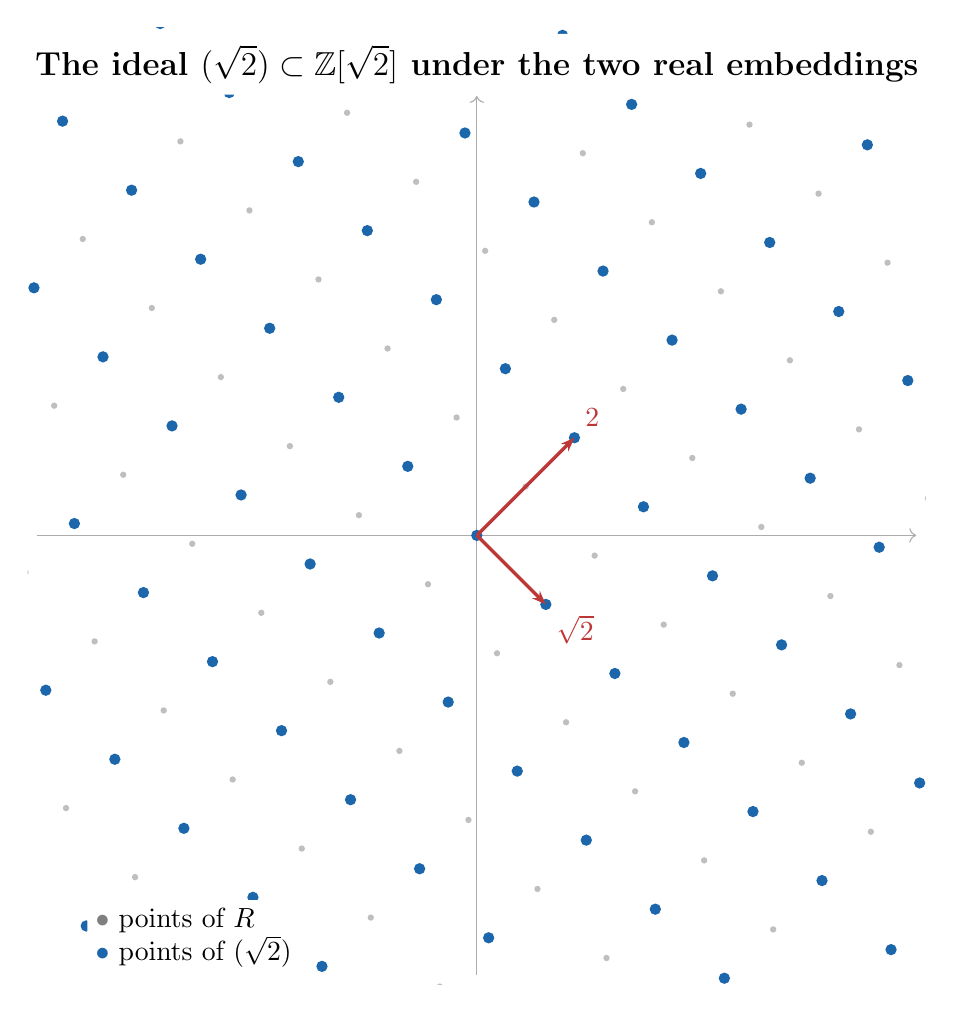
\begin{tikzpicture}[x=0.62cm,y=0.62cm]
  \clip (-9.2,-9.2) rectangle (9.2,10.4);
  \draw[->,gray!65] (-9,0)--(9,0) node[right] {$u$};
  \draw[->,gray!65] (0,-9)--(0,9) node[above] {$v$};
  \foreach \a in {-8,...,8}{
    \foreach \b in {-8,...,8}{
      \pgfmathsetmacro{\px}{\a+1.41421356*\b}
      \pgfmathsetmacro{\py}{\a-1.41421356*\b}
      \fill[gray!50] (\px,\py) circle (1.15pt);
      \pgfmathtruncatemacro{\parity}{mod(abs(\a),2)}
      \ifnum\parity=0
        \fill[idealblue] (\px,\py) circle (2.05pt);
      \fi
    }
  }
  \draw[-{Stealth[length=5pt]},basisred,very thick] (0,0)--(2,2) node[above right] {$2$};
  \draw[-{Stealth[length=5pt]},basisred,very thick] (0,0)--(1.4142,-1.4142) node[below right] {$\sqrt2$};
  \node[fill=white,rounded corners,inner sep=4pt,font=\large\bfseries] at (0,9.65) {The ideal $(\sqrt2)\subset\mathbb Z[\sqrt2]$ under the two real embeddings};
  \node[fill=white,rounded corners,inner sep=3pt,align=left] at (-5.8,-8.25) {\textcolor{gray}{\(\bullet\)} points of $R$\\\textcolor{idealblue}{\(\bullet\)} points of $(\sqrt2)$};
\end{tikzpicture}
\end{document}
